\chapter{Các phương trình Maxwell, tính hiệp biến và sóng điện từ}

\lectureoverview{Điện trường và từ trường tác dụng lên vật chất mang điện thông qua lực Lorentz, nhưng vật chất cũng phải tạo ra và sắp xếp lại các trường đó. Chúng ta sẽ phát biểu nửa đối ứng ấy của điện từ học, chỉ ra rằng các phương trình Maxwell là hiệp biến Lorentz, suy ra các nghiệm sóng của chúng, rồi đưa điện tích và dòng điện trở lại dưới một dạng làm cho sự bảo toàn địa phương trở nên tường minh. Trong suốt bài giảng, ta dùng hệ đơn vị trong đó \(c=1\).}

\section{Nửa kia của điện từ học}

Hãy bắt đầu với phần của chủ đề mà ta đã có trong tay. Nếu một hạt có điện tích \(q\) chuyển động với vận tốc \(\mathbf v\) qua điện trường và từ trường, thì lực là
\begin{equation}
\mathbf F=q\bigl(\mathbf E+\mathbf v\times\mathbf B\bigr).
\label{eq:lorentz-force-three}
\end{equation}
Thừa số \(q\) là không thể thiếu. Một hạt không mang điện không cảm nhận lực điện từ. Điện trường đóng góp ngay cả khi hạt tức thời đứng yên, còn đóng góp của từ trường thì phụ thuộc vào chuyển động của nó.

Phương trình~\eqref{eq:lorentz-force-three} cho ta biết các trường đã cho sẵn tác dụng lên vật chất như thế nào. Nó không cho ta biết điều gì quyết định các trường ấy. Điều gì tạo ra điện trường quanh một vật, từ trường quanh một vật khác, hay một sóng chuyển động qua không gian trống? Các phương trình trả lời những câu hỏi đó là các phương trình Maxwell.

\begin{figure}[H]
\centering
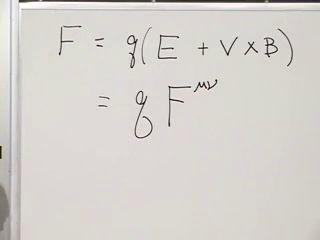
\includegraphics[width=0.62\textwidth]{lecture_58_figure_02.png}
\caption{Lực Lorentz dạng ba-vectơ và phần mở đầu của việc viết lại nó dưới dạng tensor.}
\lectureframe{00:05:49}
\end{figure}

Dạng tương đối tính của định luật lực báo trước ký hiệu mà ta sẽ cần:
\begin{equation}
f^\mu=qF^\mu{}_{\nu}u^\nu.
\label{eq:lorentz-force-four}
\end{equation}
Ở đây \(u^\nu\) là bốn-vận tốc, \(f^\mu\) là bốn-lực, và \(F^{\mu\nu}\) là một tensor phản đối xứng được ghép từ \(\mathbf E\) và \(\mathbf B\). Trên bảng lúc đầu chỉ hiển thị phần mở đầu sơ lược của biểu thức này; phép co với \(u^\nu\) cung cấp vectơ còn thiếu cần để còn lại một chỉ số lực tự do.

Có một lý do vật lý khiến vật chất phải tác dụng ngược trở lại lên trường. Một sóng điện từ có thể đập vào một điện tích, gia tốc nó và truyền năng lượng cho nó. Nếu trường có thể ảnh hưởng lên điện tích trong khi điện tích lại không bao giờ có thể ảnh hưởng lên trường, thì sẽ không có nơi nào mà năng lượng đó bị rút ra. Tác dụng và phản tác dụng chưa hẳn là toàn bộ lập luận, nhưng sự bảo toàn năng lượng khiến sự ghép đôi đối ứng ấy trở thành điều không thể tránh khỏi.

\section{Một nguồn biến thiên phát ra một nhiễu động}

Một điện tích điểm tạo ra một điện trường hướng ra ngoài hoặc vào trong tính từ vị trí của nó. Một dòng điện trong dây dẫn--một dòng các hạt mang điện--tạo ra một từ trường tuần hoàn quanh dây. Những hình ảnh tĩnh quen thuộc này đã cho thấy hai mẫu hình học khác nhau: thông lượng điện tỏa ra từ điện tích, còn các đường sức từ thì quấn quanh dòng điện.

Bây giờ hãy dịch chuyển điện tích điểm một cách đột ngột. Gần vị trí mới của nó, điện trường phải bắt đầu sắp xếp lại, nhưng một quan sát viên ở xa không thể biết được chuyển động ấy ngay tức thì. Trường cũ vẫn còn ở xa cho đến khi tín hiệu có đủ thời gian để tới nơi. Giữa vùng gần và vùng xa là một mặt lan truyền mà tại đó trường đang biến đổi. Sự sắp xếp lại đang chuyển động ấy là một nhiễu động điện từ.

Nếu điện tích bị cưỡng bức dao động qua lại, các sự sắp xếp lại kế tiếp nhau sẽ nối tiếp nhau và tạo thành một sóng điện từ. Đây là chức năng sơ đẳng của một ăng-ten: một dòng điện dao động phát nhiễu động trường ra ngoài. Đảo chiều một dòng điện trong dây cho phiên bản từ của cùng lập luận đó. Sự tuần hoàn của \(\mathbf B\) phải đảo chiều, nhưng sự đảo chiều ấy lan truyền đi thay vì xuất hiện đồng thời ở khắp nơi.

Bức tranh nhân quả này đặt ra hai mục tiêu cho các phương trình Maxwell. Chúng phải mô tả cách điện tích và dòng điện làm nguồn cho các trường, và chúng phải cho phép những biến đổi của các trường ấy lan truyền không nhanh hơn ánh sáng. Mục tiêu thứ hai đồng thời cũng là một phép kiểm tra của thuyết tương đối. Nếu các phương trình Maxwell có cùng dạng trong mọi hệ quy chiếu quán tính và hàm ý một tốc độ sóng xác định, thì mọi hệ quy chiếu quán tính đều phải suy ra cùng tốc độ đó từ chúng.

\section{Ôn lại phương trình sóng tương đối tính}

Trước khi chuyển sang các trường vectơ, hãy xét một trường vô hướng \(\phi(\mathbf x,t)\), một giá trị số tại mỗi điểm không-thời gian. Một phương trình đạo hàm bậc nhất
\begin{equation}
\partial_\mu\phi=0
\end{equation}
sẽ nói rằng mọi đạo hàm theo không-thời gian đều triệt tiêu. Khi đó trường sẽ là hằng số và vì vậy không thể mang một sóng. Một phương trình sóng tương đối tính không tầm thường dùng hai đạo hàm:
\begin{equation}
\partial_\mu\partial^\mu\phi=0.
\end{equation}
Với quy ước dấu dùng ở đây,
\begin{equation}
\left(\partial_t^2-\partial_x^2-\partial_y^2-\partial_z^2\right)\phi=0,
\label{eq:scalar-wave-four}
\end{equation}
hay, gọn hơn,
\begin{equation}
\left(\partial_t^2-\nabla^2\right)\phi=0.
\end{equation}
Lựa chọn \(c=1\) khiến thời gian và khoảng cách mang các đơn vị tương thích. Nếu khôi phục các đơn vị thông thường thì \(1/c^2\) sẽ đứng cạnh đạo hàm thời gian bậc hai.

Đối với một sóng truyền dọc theo trục \(z\), trường phụ thuộc vào \(z\) và \(t\), không phụ thuộc vào \(x\) hay \(y\). Phương trình~\eqref{eq:scalar-wave-four} rút gọn thành
\begin{equation}
\left(\partial_t^2-\partial_z^2\right)\phi=0.
\label{eq:scalar-wave-one}
\end{equation}

\begin{figure}[H]
\centering
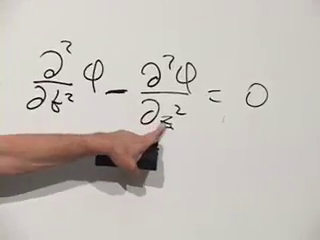
\includegraphics[width=0.56\textwidth]{lecture_58_figure_04.png}
\caption{Phương trình sóng vô hướng một chiều được dùng làm mô hình cho sóng điện từ.}
\lectureframe{00:47:03}
\end{figure}

Dạng sóng truyền tổng quát của nó là
\begin{equation}
\phi(z,t)=f(z-t)+g(z+t).
\end{equation}
Biên dạng \(f(z-t)\) chuyển động về phía \(z\) tăng, vì một điểm có pha cố định thỏa mãn \(z-t=\text{constant}\). Biên dạng \(g(z+t)\) chuyển động theo chiều ngược lại. Không có gì buộc một trong hai biên dạng phải là hình sin; bất kỳ dạng nào đủ trơn cũng tịnh tiến mà không đổi dạng.

Tuy vậy, các hàm sin vẫn thuận tiện:
\begin{equation}
\phi(z,t)=A\cos\!\bigl(k(z-t)\bigr).
\end{equation}
Số sóng \(k\) quyết định bước sóng,
\begin{equation}
\lambda=\frac{2\pi}{k}.
\end{equation}
\(k\) lớn tạo ra dao động không gian nhanh và bước sóng ngắn; \(k\) nhỏ tạo ra bước sóng dài. Những biên dạng này ngay sau đây sẽ trở thành các thành phần của \(\mathbf E\) và \(\mathbf B\).

\section{Giải tích vectơ mà Maxwell cần dùng}

Các phương trình Maxwell được viết bằng tích vô hướng, tích có hướng, độ phân kỳ và độ xoáy. Đáng để dựng lại hệ ký hiệu này một lần, vì các phép tính theo thành phần về sau dùng đúng chính những mẫu đó.

Đối với các ba-vectơ thông thường \(\mathbf a\) và \(\mathbf b\), tích vô hướng là vô hướng
\begin{equation}
\mathbf a\cdot\mathbf b
=a_xb_x+a_yb_y+a_zb_z.
\end{equation}
Tích có hướng là một vectơ khác,
\begin{align}
(\mathbf a\times\mathbf b)_x&=a_yb_z-a_zb_y,\\
(\mathbf a\times\mathbf b)_y&=a_zb_x-a_xb_z,\\
(\mathbf a\times\mathbf b)_z&=a_xb_y-a_yb_x.
\end{align}
Các thành phần còn lại tuân theo thứ tự tuần hoàn \(x\to y\to z\to x\).

Hãy đưa vào toán tử vi phân
\begin{equation}
\boldsymbol\nabla=
\left(\partial_x,\partial_y,\partial_z\right).
\end{equation}
Các phần tử của nó là các toán tử chứ không phải các số thông thường, nhưng vẫn có thể dùng các mẫu tích vô hướng và tích có hướng. Với một trường vectơ \(\mathbf A\),
\begin{equation}
\boldsymbol\nabla\cdot\mathbf A
=\partial_xA_x+\partial_yA_y+\partial_zA_z
\label{eq:divergence}
\end{equation}
là độ phân kỳ, còn
\begin{align}
(\boldsymbol\nabla\times\mathbf A)_x
 &=\partial_yA_z-\partial_zA_y,\\
(\boldsymbol\nabla\times\mathbf A)_y
 &=\partial_zA_x-\partial_xA_z,\\
(\boldsymbol\nabla\times\mathbf A)_z
 &=\partial_xA_y-\partial_yA_x
\label{eq:curl}
\end{align}
là các thành phần của độ xoáy.

Hình học cũng quan trọng như các công thức. Một trường vectơ có độ phân kỳ dương ở nơi nó có vẻ chảy ra ngoài từ một nguồn. Nó có độ xoáy ở nơi nó tuần hoàn. Điện trường hướng tâm của một điện tích điểm minh họa độ phân kỳ; từ trường quấn quanh một dây dẫn có dòng điện minh họa độ xoáy. Một trường vectơ không đổi theo không gian thì không có phân kỳ lẫn xoáy.

\section{Các phương trình Maxwell trong chân không}

Khi không có điện tích và dòng điện, các phương trình Maxwell là
\begin{align}
\boldsymbol\nabla\times\mathbf E&=-\partial_t\mathbf B,
\label{eq:faraday-vac}\\
\boldsymbol\nabla\cdot\mathbf B&=0,
\label{eq:gauss-b-vac}\\
\boldsymbol\nabla\times\mathbf B&=\partial_t\mathbf E,
\label{eq:ampere-vac}\\
\boldsymbol\nabla\cdot\mathbf E&=0.
\label{eq:gauss-e-vac}
\end{align}
Hai phương trình xoáy gần như hoán đổi \(\mathbf E\) và \(\mathbf B\), nhưng một dấu trừ thiết yếu phân biệt chúng. Hai phương trình phân kỳ nói rằng cả hai trường đều không có nguồn trong miền chân không đang xét. Độ phân kỳ từ vẫn bằng không ngay cả sau khi khôi phục các nguồn điện; điện từ học thông thường không có điện tích từ.

\begin{figure}[H]
\centering
\includegraphics[width=0.76\textwidth]{lecture_58_figure_06.png}
\caption{Bốn phương trình Maxwell trong chân không, được sắp xếp để bộc lộ tính đối xứng gần đúng giữa điện trường và từ trường.}
\lectureframe{00:27:30}
\end{figure}

Mật độ điện tích \(\rho\) rốt cuộc sẽ thay số 0 ở vế phải của Phương trình~\eqref{eq:gauss-e-vac}, và mật độ dòng điện \(\mathbf J\) sẽ đi vào Phương trình~\eqref{eq:ampere-vac}. Tạm thời ta hoãn các hạng đó lại. Các phương trình không nguồn bộc lộ cấu trúc biến đổi và cơ chế sóng với mức rườm rà ít nhất.

Chúng cũng làm sắc nét nghịch đề của Einstein. Một quan sát viên Galile đi theo một sóng sẽ mong đợi trừ các vận tốc và đo được một tốc độ sóng nhỏ hơn. Thế nhưng nếu cùng các phương trình Maxwell đúng trong mọi hệ quy chiếu quán tính, thì mỗi quan sát viên đều suy ra cùng một tốc độ sóng đơn vị. Lối thoát không phải là thay đổi phương trình sóng từ hệ này sang hệ khác. Mà là dùng phép biến đổi Lorentz và biểu diễn các phương trình Maxwell bằng những đối tượng mà các quy luật biến đổi của chúng đã được biết sẵn.

\section{Điện trường và từ trường trong một tensor duy nhất}

Điện trường và từ trường kết hợp thành tensor trường phản đối xứng
\begin{equation}
F^{\mu\nu}=
\begin{pmatrix}
0   & -E_x & -E_y & -E_z\\
E_x & 0    & -B_z & B_y\\
E_y & B_z  & 0    & -B_x\\
E_z & -B_y & B_x  & 0
\end{pmatrix},
\label{eq:l0203-field-tensor}
\end{equation}
trong đó thứ tự hàng và cột là \(t,x,y,z\). Tính phản đối xứng,
\begin{equation}
F^{\mu\nu}=-F^{\nu\mu},
\end{equation}
buộc các phần tử trên đường chéo phải triệt tiêu và xác định nửa dưới của ma trận từ nửa trên. Các phần tử thời gian-không gian chứa \(\mathbf E\); các phần tử thuần không gian chứa \(\mathbf B\).

\begin{figure}[H]
\centering
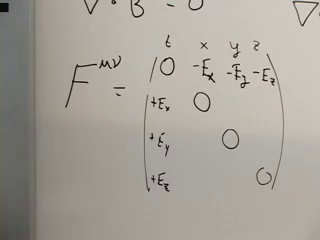
\includegraphics[width=0.58\textwidth]{lecture_58_figure_03.png}
\caption{Tensor trường điện từ hoàn chỉnh, bao gồm các phần tử điện và từ của nó.}
\lectureframe{00:32:05}
\end{figure}

Tầm quan trọng của \(F^{\mu\nu}\) không chỉ là việc sáu thành phần trường vừa khít trong một ma trận. Dưới một phép biến đổi Lorentz, nó biến đổi như một tensor hạng hai. Vì thế điện trường và từ trường do các quan sát viên khác nhau đo được trộn lẫn đúng theo cách cần thiết để toàn bộ đối tượng biến đổi một cách nhất quán.

Có một tensor phản đối xứng thứ hai, tensor trường đối ngẫu \(\widetilde F^{\mu\nu}\). Với quy ước hiện tại, nó thu được từ Phương trình~\eqref{eq:l0203-field-tensor} qua phép thay thế
\begin{equation}
\mathbf E\longmapsto-\mathbf B,
\qquad
\mathbf B\longmapsto\mathbf E.
\label{eq:dual-replacement}
\end{equation}
Do đó
\begin{equation}
\widetilde F^{\mu\nu}=
\begin{pmatrix}
0    & B_x  & B_y  & B_z\\
-B_x & 0    & -E_z & E_y\\
-B_y & E_z  & 0    & -E_x\\
-B_z & -E_y & E_x  & 0
\end{pmatrix}.
\label{eq:dual-tensor}
\end{equation}
Dấu trong Phương trình~\eqref{eq:dual-replacement} là quan trọng. Bài giảng trước hết thử phát biểu phép hoán đổi ấy bằng lời, nhận ra sự không khớp về dấu, rồi sửa lại trước khi hoàn tất ma trận.

\begin{figure}[H]
\centering
\includegraphics[width=0.58\textwidth]{lecture_58_figure_07.png}
\caption{Tensor đối ngẫu đang được dựng bằng cách hoán đổi các phần tử điện và từ với dấu thích hợp.}
\lectureframe{00:35:45}
\end{figure}

\section{Các phương trình chân không hiệp biến}

Mỗi phương trình Maxwell chứa một đạo hàm. Bắt đầu từ một tensor hạng hai và co một chỉ số đạo hàm thì còn lại một chỉ số tự do, nên các ứng viên hiệp biến tự nhiên là
\begin{align}
\partial_\mu F^{\mu\nu}&=0,
\label{eq:maxwell-covariant-vac}\\
\partial_\mu\widetilde F^{\mu\nu}&=0.
\label{eq:maxwell-dual-vac}
\end{align}
Với mỗi giá trị cố định của \(\nu\), Phương trình~\eqref{eq:maxwell-covariant-vac} là một phương trình. Vì \(\nu\) có thể là \(t,x,y,z\), nó gộp bốn phương trình vô hướng. Phương trình~\eqref{eq:maxwell-dual-vac} gộp bốn phương trình còn lại. Điều này khớp với hai phương trình vectơ về độ xoáy và hai phương trình vô hướng về độ phân kỳ trong danh sách ban đầu.

Ký hiệu gọn chỉ hữu ích nếu nó tái tạo được các phương trình quen thuộc. Lấy \(\nu=z\):
\begin{align}
\partial_\mu F^{\mu z}
&=\partial_tF^{tz}
  +\partial_xF^{xz}
  +\partial_yF^{yz}
  +\partial_zF^{zz}\\
&=-\partial_tE_z+\partial_xB_y-\partial_yB_x\\
&=-\partial_tE_z+
  \bigl(\boldsymbol\nabla\times\mathbf B\bigr)_z.
\end{align}
Hạng \(F^{zz}\) triệt tiêu do tính phản đối xứng. Cho kết quả bằng không thì ta được thành phần \(z\) của
\begin{equation}
\boldsymbol\nabla\times\mathbf B=\partial_t\mathbf E.
\end{equation}
Các thành phần \(x\) và \(y\) suy ra bằng cách quay vòng các chỉ số.

\begin{figure}[H]
\centering
\includegraphics[width=0.76\textwidth]{lecture_58_figure_08.png}
\caption{Khai triển theo thành phần của phương trình trường hiệp biến; phần tử tensor trên đường chéo triệt tiêu và các hạng còn lại tái dựng các phương trình Maxwell.}
\lectureframe{00:43:30}
\end{figure}

Bây giờ lấy thành phần thời gian:
\begin{align}
\partial_\mu F^{\mu t}
&=\partial_tF^{tt}
  +\partial_xF^{xt}
  +\partial_yF^{yt}
  +\partial_zF^{zt}\\
&=\partial_xE_x+\partial_yE_y+\partial_zE_z\\
&=\boldsymbol\nabla\cdot\mathbf E.
\end{align}
Vì vậy nó cho Phương trình~\eqref{eq:gauss-e-vac}. Thực hiện cùng những phép kiểm tra đó trên tensor đối ngẫu cho ra
\(\boldsymbol\nabla\cdot\mathbf B=0\) và
\(\boldsymbol\nabla\times\mathbf E=-\partial_t\mathbf B\).

Giờ đây các phương trình gọn đã được thiết lập chứ không còn chỉ là phỏng đoán. Cấu trúc chỉ số tự do của chúng khiến chúng là các phương trình bốn-vectơ, nên một phép biến đổi Lorentz làm thay đổi các thành phần của chúng nhưng không làm thay đổi dạng của chúng. Đây là nghĩa chính xác mà theo đó các phương trình Maxwell trong chân không là như nhau trong mọi hệ quy chiếu quán tính.

\section{Từ các phương trình bậc nhất đến một sóng}

Các phương trình Maxwell chỉ chứa các đạo hàm bậc nhất, trong khi một phương trình sóng chứa các đạo hàm bậc hai. Sự không khớp bề ngoài này được giải quyết vì lý thuyết Maxwell ghép cặp hai trường. Một cặp phương trình bậc nhất cho \(\mathbf E\) và \(\mathbf B\) có thể được kết hợp thành một phương trình bậc hai chỉ cho riêng một trong hai trường.

Lấy đạo hàm theo thời gian của Phương trình~\eqref{eq:ampere-vac}:
\begin{equation}
\partial_t^2\mathbf E
=\boldsymbol\nabla\times\partial_t\mathbf B.
\end{equation}
Định luật Faraday cung cấp đạo hàm theo thời gian của \(\mathbf B\),
\begin{equation}
\partial_t\mathbf B=-\boldsymbol\nabla\times\mathbf E,
\end{equation}
và do đó
\begin{equation}
\partial_t^2\mathbf E
=-\boldsymbol\nabla\times
  \bigl(\boldsymbol\nabla\times\mathbf E\bigr).
\label{eq:double-curl}
\end{equation}

Trên bảng người ta triển khai một thành phần thay vì viện dẫn một đồng nhất thức đã học thuộc. Với thành phần \(x\),
\begin{align}
\bigl[\boldsymbol\nabla\times
(\boldsymbol\nabla\times\mathbf E)\bigr]_x
&=\partial_y(\boldsymbol\nabla\times\mathbf E)_z
 -\partial_z(\boldsymbol\nabla\times\mathbf E)_y\\
&=\partial_y(\partial_xE_y-\partial_yE_x)\\
&\quad-\partial_z(\partial_zE_x-\partial_xE_z)\\
&=\partial_x(\partial_yE_y+\partial_zE_z)
 -\partial_y^2E_x\\
&\quad-\partial_z^2E_x.
\end{align}
Cộng rồi trừ \(\partial_x^2E_x\) để làm lộ ra độ phân kỳ:
\begin{align}
\bigl[\boldsymbol\nabla\times
(\boldsymbol\nabla\times\mathbf E)\bigr]_x
&=\partial_x(\boldsymbol\nabla\cdot\mathbf E)
 -\nabla^2E_x.
\label{eq:double-curl-x}
\end{align}
Trong chân không \(\boldsymbol\nabla\cdot\mathbf E=0\). Kết hợp
Phương trình~\eqref{eq:double-curl} và \eqref{eq:double-curl-x} cho
\begin{equation}
\left(\partial_t^2-\nabla^2\right)E_x=0.
\label{eq:ex-wave}
\end{equation}

\begin{figure}[H]
\centering
\includegraphics[width=0.72\textwidth]{lecture_58_figure_09.png}
\caption{Phép tính theo thành phần đi tới phương trình sóng cho \(E_x\).}
\lectureframe{00:57:10}
\end{figure}

Phép tính tương tự cũng áp dụng cho \(E_y\) và \(E_z\), và một phép khử tương tự cho ta
\begin{equation}
\left(\partial_t^2-\nabla^2\right)\mathbf B=0.
\end{equation}
Vì vậy, điện trường và từ trường có thể lan truyền trong không gian trống dưới dạng sóng. Trong hệ đơn vị dùng ở đây, tốc độ của chúng bằng một, nghĩa là tốc độ ấy là \(c\) khi khôi phục các đơn vị thông thường.

\section{Một sóng phẳng và sự phân cực của nó}

Xây dựng một sóng đơn giản truyền theo chiều dương của \(z\):
\begin{equation}
\mathbf E(z,t)
=\widehat{\mathbf x}\,E_0
  \cos\!\bigl(k(z-t)\bigr).
\label{eq:plane-e}
\end{equation}
Biên dạng của nó tịnh tiến dọc theo \(z\) mà không đổi dạng. Vì điện trường hướng theo trục \(x\), nên sóng được phân cực thẳng theo phương \(x\). Ta chọn \(E_y=0\) chỉ để giữ cho ví dụ đơn giản; cũng có thể đưa vào một phân cực ngang thứ hai.

Thành phần dọc không tự do theo cùng cách. Vì sóng chỉ phụ thuộc vào \(z\) và \(t\),
\begin{equation}
\boldsymbol\nabla\cdot\mathbf E
=\partial_zE_z=0.
\end{equation}
Do đó \(E_z\) có thể là một hằng số, nhưng nó không thể chứa biên dạng sóng biến thiên. Một trường nền đồng đều có thể được chồng thêm vào hoặc bỏ đi một cách độc lập; nó không phải là một phần của bức xạ đang lan truyền. Bản thân sóng là ngang:
\begin{equation}
\mathbf E_{\mathrm{wave}}\cdot\widehat{\mathbf z}=0.
\end{equation}

Định luật Faraday xác định từ trường. Đối với Phương trình~\eqref{eq:plane-e}, thành phần khác không duy nhất của \(\boldsymbol\nabla\times\mathbf E\) là thành phần \(y\),
\begin{equation}
(\boldsymbol\nabla\times\mathbf E)_y=\partial_zE_x.
\end{equation}
Do đó \(\partial_t\mathbf B\) hướng theo \(y\), và một lựa chọn tương thích là
\begin{equation}
\mathbf B(z,t)
=\widehat{\mathbf y}\,E_0
  \cos\!\bigl(k(z-t)\bigr).
\label{eq:plane-b}
\end{equation}
Trong hệ đơn vị này, biên độ điện trường và từ trường bằng nhau. Hướng của chúng tuân theo
\begin{equation}
\mathbf E\perp\mathbf B,
\qquad
\mathbf E\perp\widehat{\mathbf z},
\qquad
\mathbf B\perp\widehat{\mathbf z},
\qquad
\mathbf E\times\mathbf B\parallel\widehat{\mathbf z}.
\end{equation}

\begin{figure}[H]
\centering
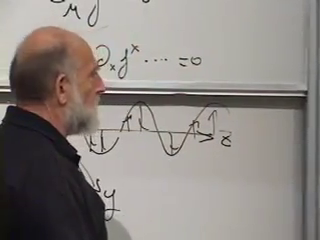
\includegraphics[width=0.70\textwidth]{lecture_58_figure_05.png}
\caption{Hình phác hoàn chỉnh trên bảng của một sóng điện từ ngang: các dao động của điện trường và từ trường vuông góc với nhau và với phương truyền.}
\lectureframe{01:05:25}
\end{figure}

\begin{figure}[H]
\centering
\scalebox{0.90}{%
\begin{tikzpicture}[x=1cm,y=1cm,>=Latex]
  \draw[->,thick] (0,0) -- (8.2,0) node[right] {$z$};
  \draw[->,thick] (0,-1.6) -- (0,1.7) node[above] {$x$};
  \draw[->,thick] (0,0) -- (-1.15,-0.8) node[below left] {$y$};
  \draw[blue!70!black,thick,domain=0:7.5,samples=120]
    plot (\x,{0.95*sin(90*\x)});
  \foreach \z/\s in {0.8/1,2.8/-1,4.8/1,6.8/-1}{
    \draw[->,green!45!black,thick]
      (\z,0) -- ++({-0.55*\s},{-0.38*\s});
  }
  \node[blue!70!black] at (6.9,1.25) {$\mathbf E$};
  \node[green!45!black] at (5.2,-1.05) {$\mathbf B$};
  \draw[->,very thick] (6.2,1.55) -- (7.7,1.55)
    node[midway,above] {propagation};
\end{tikzpicture}
}
\caption{Các trường \(\mathbf E\) và \(\mathbf B\) vuông góc với nhau và với phương truyền.}
\end{figure}

Đó là bản chất của ánh sáng và của mọi bức xạ điện từ trong chân không. Vì các phương trình đã sinh ra sóng này là hiệp biến Lorentz, nên một quan sát viên quán tính khác vẫn sẽ mô tả một sóng điện từ lan truyền với tốc độ \(c\), với điện trường và từ trường ngang.

\section{Mật độ điện tích và mật độ dòng điện}

Bây giờ ta khôi phục các nguồn đã tạm thời gác sang một bên. Khi nhiều hạt mang điện chiếm một vùng, sẽ hữu ích nếu thô hạt hóa chúng thành một mật độ điện tích liên tục
\begin{equation}
\rho(\mathbf x,t)=\frac{dQ}{dV}.
\end{equation}
Phép gần đúng này giống như việc coi nước là một chất lưu liên tục mặc dù nó được tạo thành từ các phân tử. Các điện tích dương và âm đóng góp với dấu ngược nhau, nên \(\rho\) là điện tích thuần trên một đơn vị thể tích.

Điện tích trong một vùng \(V\) được chọn là
\begin{equation}
Q_V(t)=\int_V\rho(\mathbf x,t)\,dV.
\label{eq:charge-volume}
\end{equation}
Mật độ ấy có thể biến thiên theo vị trí và thời gian. Một khối điện tích có thể rời khỏi một điểm, làm thay đổi mật độ cục bộ ở đó. Tuy nhiên, nó không thể biến thiên một cách tùy ý. Trong tự nhiên, điện tích được bảo toàn.

Chỉ bảo toàn toàn cục thôi thì còn quá yếu. Nó sẽ cho phép điện tích biến mất khỏi Trái Đất và đồng thời xuất hiện lại trên Sao Hỏa trong khi tổng điện tích vẫn không đổi. Phát biểu mạnh hơn là phát biểu cục bộ: điện tích chỉ có thể rời khỏi một nơi và đến một nơi khác thông qua một dòng chảy trong khoảng không gian xen giữa.

Để mô tả dòng chảy đó, hãy lấy một phần tử diện tích có hướng vi phân
\begin{equation}
d\boldsymbol\sigma=\widehat{\mathbf n}\,d\sigma.
\end{equation}
Độ lớn của nó là diện tích, còn hướng của nó là pháp tuyến với bề mặt. Mật độ dòng điện \(\mathbf J\) được định nghĩa sao cho điện tích đi qua phần tử ấy trong một đơn vị thời gian là
\begin{equation}
\frac{dQ}{dt}=\mathbf J\cdot d\boldsymbol\sigma.
\label{eq:current-flux-element}
\end{equation}
Độ lớn của \(\mathbf J\) là điện tích trên một đơn vị diện tích trong một đơn vị thời gian, còn hướng của nó là hướng dòng chảy của điện tích dương.

\begin{figure}[H]
\centering
\includegraphics[width=0.64\textwidth]{lecture_58_figure_10.png}
\caption{Một phần tử diện tích có hướng và thừa số thông lượng \(d\boldsymbol\sigma\cdot\mathbf J\).}
\lectureframe{01:18:15}
\end{figure}

Tích vô hướng chọn ra thành phần pháp tuyến với bề mặt. Một dòng điện tiếp tuyến với bề mặt không đi qua phía nào cả và đóng góp bằng không. Với độ lớn cố định, một dòng điện song song với pháp tuyến cho thông lượng lớn nhất. Dòng điện trong dây là một trường hợp đặc biệt, nhưng \(\mathbf J\) cũng có thể mô tả điện tích chảy qua một tấm hoặc khắp không gian ba chiều.

\section{Bảo toàn cục bộ và phương trình liên tục}

Giữ cố định một vùng \(V\) trong không gian và cho mọi phần tử trên biên kín \(\partial V\) của nó hướng ra ngoài. Nếu có dòng điện thuần hướng ra ngoài, thì điện tích bên trong giảm:
\begin{equation}
\frac{dQ_V}{dt}
=-\oint_{\partial V}\mathbf J\cdot d\boldsymbol\sigma.
\label{eq:integral-conservation}
\end{equation}
Dấu trừ là vật lý chứ không phải quy ước: thông lượng dương hướng ra ngoài lấy điện tích dương ra khỏi vùng ấy. Dùng Phương trình~\eqref{eq:charge-volume},
\begin{equation}
\int_V\partial_t\rho\,dV
=-\oint_{\partial V}\mathbf J\cdot d\boldsymbol\sigma.
\label{eq:integral-continuity-one}
\end{equation}

\begin{figure}[H]
\centering
\includegraphics[width=0.72\textwidth]{lecture_58_figure_11.png}
\caption{Định luật bảo toàn cho một vùng cố định sau khi thông lượng qua mặt được chuyển thành một phát biểu theo thể tích.}
\lectureframe{01:29:00}
\end{figure}

Định lý Gauss, còn gọi là định lý phân kỳ, liên hệ thông lượng qua một mặt kín với phân kỳ trong phần bên trong của nó:
\begin{equation}
\oint_{\partial V}\mathbf A\cdot d\boldsymbol\sigma
=\int_V\boldsymbol\nabla\cdot\mathbf A\,dV.
\label{eq:divergence-theorem}
\end{equation}
Ta có thể hình dung những ống ẩn bơm nước vào tại các điểm bên trong một bình chứa. Phân kỳ đo tốc độ cục bộ mà tại đó nước đi ra khỏi các đầu ống; tích phân mặt đo tổng lượng nước rời khỏi bình. Bất cứ thứ gì được tạo ra dưới dạng dòng chảy hướng ra ngoài ở bên trong cuối cùng cũng phải đi qua biên.

Áp dụng Phương trình~\eqref{eq:divergence-theorem} cho \(\mathbf J\) ta được
\begin{equation}
\int_V
\left(\partial_t\rho+\boldsymbol\nabla\cdot\mathbf J\right)dV=0.
\end{equation}
Hệ thức này đúng với mọi vùng \(V\) có thể chọn. Vì vậy, hàm dưới dấu tích phân phải triệt tiêu tại từng điểm:
\begin{equation}
\boxed{\partial_t\rho+\boldsymbol\nabla\cdot\mathbf J=0.}
\label{eq:continuity-three}
\end{equation}

\begin{figure}[H]
\centering
\includegraphics[width=0.72\textwidth]{lecture_58_figure_12.png}
\caption{Phương trình liên tục cục bộ được viết theo từng thành phần.}
\lectureframe{01:29:50}
\end{figure}

Phương trình~\eqref{eq:continuity-three} phát biểu đúng chính điều mà bảo toàn cục bộ đòi hỏi. Nếu mật độ điện tích giảm tại một điểm hoặc trong một vùng nhỏ, thì dòng điện phải phân kỳ ra ngoài từ đó. Nếu dòng điện hội tụ vào trong, mật độ điện tích tăng lên.

Mật độ và dòng điện kết hợp một cách tự nhiên thành bốn-dòng điện
\begin{equation}
J^\mu=(\rho,J_x,J_y,J_z)
\label{eq:four-current}
\end{equation}
trong hệ đơn vị \(c=1\). Phương trình liên tục trở thành phương trình vô hướng Lorentz
\begin{equation}
\partial_\mu J^\mu=0.
\label{eq:continuity-four}
\end{equation}
Dòng chảy của một phân bố tương đối tính phải biến đổi như một bốn-vectơ, cũng như bốn-vận tốc của một hạt đơn lẻ. Phương trình~\eqref{eq:continuity-four} làm cho bảo toàn điện tích cục bộ có hiệu lực trong mọi hệ quy chiếu quán tính.

\section{Các phương trình Maxwell có nguồn}

Khôi phục điện tích và dòng điện thì ta có
\begin{align}
\boldsymbol\nabla\cdot\mathbf E&=\rho,
\label{eq:gauss-e-source}\\
\boldsymbol\nabla\cdot\mathbf B&=0,\\
\boldsymbol\nabla\times\mathbf E&=-\partial_t\mathbf B,\\
\boldsymbol\nabla\times\mathbf B&=\partial_t\mathbf E+\mathbf J.
\label{eq:ampere-source}
\end{align}
Các phương trình có chứa nguồn điện gộp lại thành
\begin{equation}
\boxed{\partial_\mu F^{\mu\nu}=J^\nu,}
\label{eq:maxwell-source-covariant}
\end{equation}
trong khi cặp phương trình từ không nguồn vẫn là
\begin{equation}
\boxed{\partial_\mu\widetilde F^{\mu\nu}=0.}
\label{eq:maxwell-dual-source}
\end{equation}

\begin{figure}[H]
\centering
\includegraphics[width=0.78\textwidth]{lecture_58_figure_13.png}
\caption{Các phương trình Maxwell có nguồn đặt bên cạnh dạng hiệp biến của chúng \(\partial_\mu F^{\mu\nu}=J^\nu\).}
\lectureframe{01:34:00}
\end{figure}

Thành phần thời gian của Phương trình~\eqref{eq:maxwell-source-covariant} là
\begin{equation}
\partial_\mu F^{\mu t}=J^t=\rho,
\end{equation}
và phép tính theo thành phần đã thực hiện trước đó biến vế trái của nó thành
\(\boldsymbol\nabla\cdot\mathbf E\). Ba thành phần không gian cho lại
\(\boldsymbol\nabla\times\mathbf B=\partial_t\mathbf E+\mathbf J\).

Cũng có một phép kiểm tra tính nhất quán hữu ích. Cho \(\partial_\nu\) tác dụng lên
Phương trình~\eqref{eq:maxwell-source-covariant} thì được
\begin{equation}
\partial_\nu J^\nu
=\partial_\nu\partial_\mu F^{\mu\nu}=0,
\end{equation}
vì hai đạo hàm là đối xứng dưới \(\mu\leftrightarrow\nu\), còn \(F^{\mu\nu}\) thì phản đối xứng.\editorialnote{Phép kiểm tra ngắn gọn về tính nhất quán này suy ra từ phương trình hiệp biến và làm rõ vì sao các phương trình Maxwell có nguồn tự động tuân theo phương trình liên tục.}

Cấu trúc tương hỗ giờ đây đã hoàn chỉnh. Định luật lực tensor \(f^\mu=qF^\mu{}_\nu u^\nu\) mô tả cách các trường tác dụng lên điện tích, còn Phương trình~\eqref{eq:maxwell-source-covariant} mô tả cách điện tích và dòng điện sinh ra các trường. Cả hai đều là các phương trình tensor. Trong chân không, chính các phương trình trường ấy cho ra các sóng ngang lan truyền với tốc độ \(c\). Vì vậy, hiệp biến Lorentz và phương trình sóng điện từ gặp nhau đúng tại điểm đã thúc đẩy việc xây dựng này: mọi quan sát viên quán tính đều thu được cùng những định luật điện từ học và cùng một tốc độ ánh sáng.